\documentclass[applsci,article,submit,oneauthor,pdftex]{Definitions/mdpi}

\firstpage{1}
\pubvolume{xx}
\issuenum{1}
\articlenumber{xx}
\pubyear{2026}
\copyrightyear{2026}
\Title{Auditing Protocol-Dependent Performance and Compound-Fault Recovery under Sealed Evaluation}
\newcommand{\orcidauthorA}{0009-0008-4941-5641}
\Author{Zixuan Liu\orcidA{}}
\AuthorNames{Zixuan Liu}
\address{Hubei University of Technology, Wuhan, China}
\corres{Correspondence: 2411621306@hbut.edu.cn}
\abstract{Source-domain evaluations can overstate transportability-oriented compound fault recognition when physical units are not separated or compound labels influence model selection. We introduce the Sealed Compound Generalization Protocol (SCGP), which separates development, nested physical-unit selection, and one-shot sealed confirmation without introducing a new classifier. A new \texorpdfstring{2$\times$2}{2x2} audit of the HANOI HUST bearing archive crossed split hierarchy with endpoint aggregation. The fixed logistic--envelope reference yielded record-level/bearing-aggregated AUROC and exact-set values of 0.951/0.776 and 0.959/0.791 under record-grouped splitting, and 0.828/0.510 and 0.860/0.490 under bearing-grouped splitting. A separate nested-selected-candidate evaluation under the bearing-grouped outer protocol yielded 0.777/0.420 and 0.803/0.406, with fold-specific model identities. These endpoint values were associated with different registered split and aggregation contracts; they do not establish a general aggregation improvement or universal estimator invariance. In a one-shot Paderborn lockbox containing three physical bearing codes, the frozen reference achieved exact-set accuracy of 1/3 at the bearing-code level; this is treated as a small-sample boundary case, not as universal cross-rig failure.}
\keyword{machinery fault recognition; sealed confirmation; protocol sensitivity; selection instability; physical-unit split}

\usepackage{amssymb}
\usepackage{xcolor}
\newcommand{\tbl}[1]{\textcolor{blue}{Table~#1}}
\newcommand{\fig}[1]{\textcolor{blue}{Figure~#1}}

\begin{document}

\section{Introduction}

Deployed machinery diagnostics must generalize across physical units, operating states, and fault compositions not observed during development. This requirement is especially important for compound-fault decisions: identifying one damaged component is not equivalent to recovering the complete fault set needed for maintenance planning and risk control. The HUST bearing dataset supports diagnosis studies under varied fault and operating conditions \cite{r01}. A subsequent comparison showed that apparent performance also depends on the representation and learning model \cite{r02}.

Method development has advanced quickly, but evaluation design has not always received equal attention. A systematic review identifies transfer learning as a major route for coping with distribution changes in machinery diagnosis \cite{r03}. More directly, a recent study demonstrates that leakage between vibration-signal partitions can materially inflate bearing-diagnosis results \cite{r32}. Domain-generalization surveys likewise show that datasets, domain definitions, and validation protocols remain heterogeneous across the field \cite{r33}. A rotating-machinery-specific survey reaches a similar conclusion for cross-condition generalization \cite{r34}.

These observations distinguish model performance from evidential status. Window- or record-level splits can retain dependence between training and evaluation samples. A model selected under one physical-unit partition may also lose preference under another. Finally, confirmation labels invalidate one-shot evaluation if they influence representation or model selection. Existing studies often optimize the classifier while leaving these evaluation permissions implicit, making it difficult to determine whether a reported score reflects a transportable fault signal or a favorable protocol.

We therefore propose the sealed compound generalization protocol (SCGP), which formalizes and operationalizes physical-unit partitioning, nested model selection, and one-shot sealed compound confirmation as an auditable evaluation contract. The contribution is an operational framework and an empirical audit of its consequences on the registered archive, not a new classifier, statistical theory, or generalization algorithm.

We ask how reported performance changes as evaluation moves from random partitions to physical-unit separation. We also test whether nested selection repeatedly favors the same model--representation pair. Finally, we assess whether a frozen configuration retains component-level and exact-set performance after one-shot compound-label opening.

The resulting contribution is a bounded evaluation claim: if performance changes as unit independence and label secrecy are strengthened, then the source score should be reported as a protocol-bound reference rather than a deployment guarantee. We support this claim with matched G2 protocol cells, a pre-specified G3 model-family audit, sealed HANOI HUST confirmation, and a deliberately limited Paderborn cross-rig boundary check. Any selection-instability observation is empirical for the registered HANOI candidate space, not a general property of nested selection.

The contributions of this study are threefold. First, we define SCGP as a reproducible evaluation contract that separates physical-unit independence, nested model selection, and sealed compound confirmation. Second, we quantify the performance and selection changes produced by progressively stricter access states on the HANOI HUST bearing archive, while auditing whether the effect persists across engineered and raw-waveform model families. Third, we perform a one-shot external boundary check on Paderborn and report its negative result without interpreting it as universal cross-dataset failure. The practical implication is that machinery diagnosis should report component-level discrimination and exact-set recovery together, and should distinguish a source-domain reference from a deployment guarantee.

\fig{\ref{fig:scgp_access_ladder}} summarizes the access progression, and \tbl{\ref{tab:scgp-positioning}} formalizes the corresponding contract.

\begin{figure}[H]
\centering
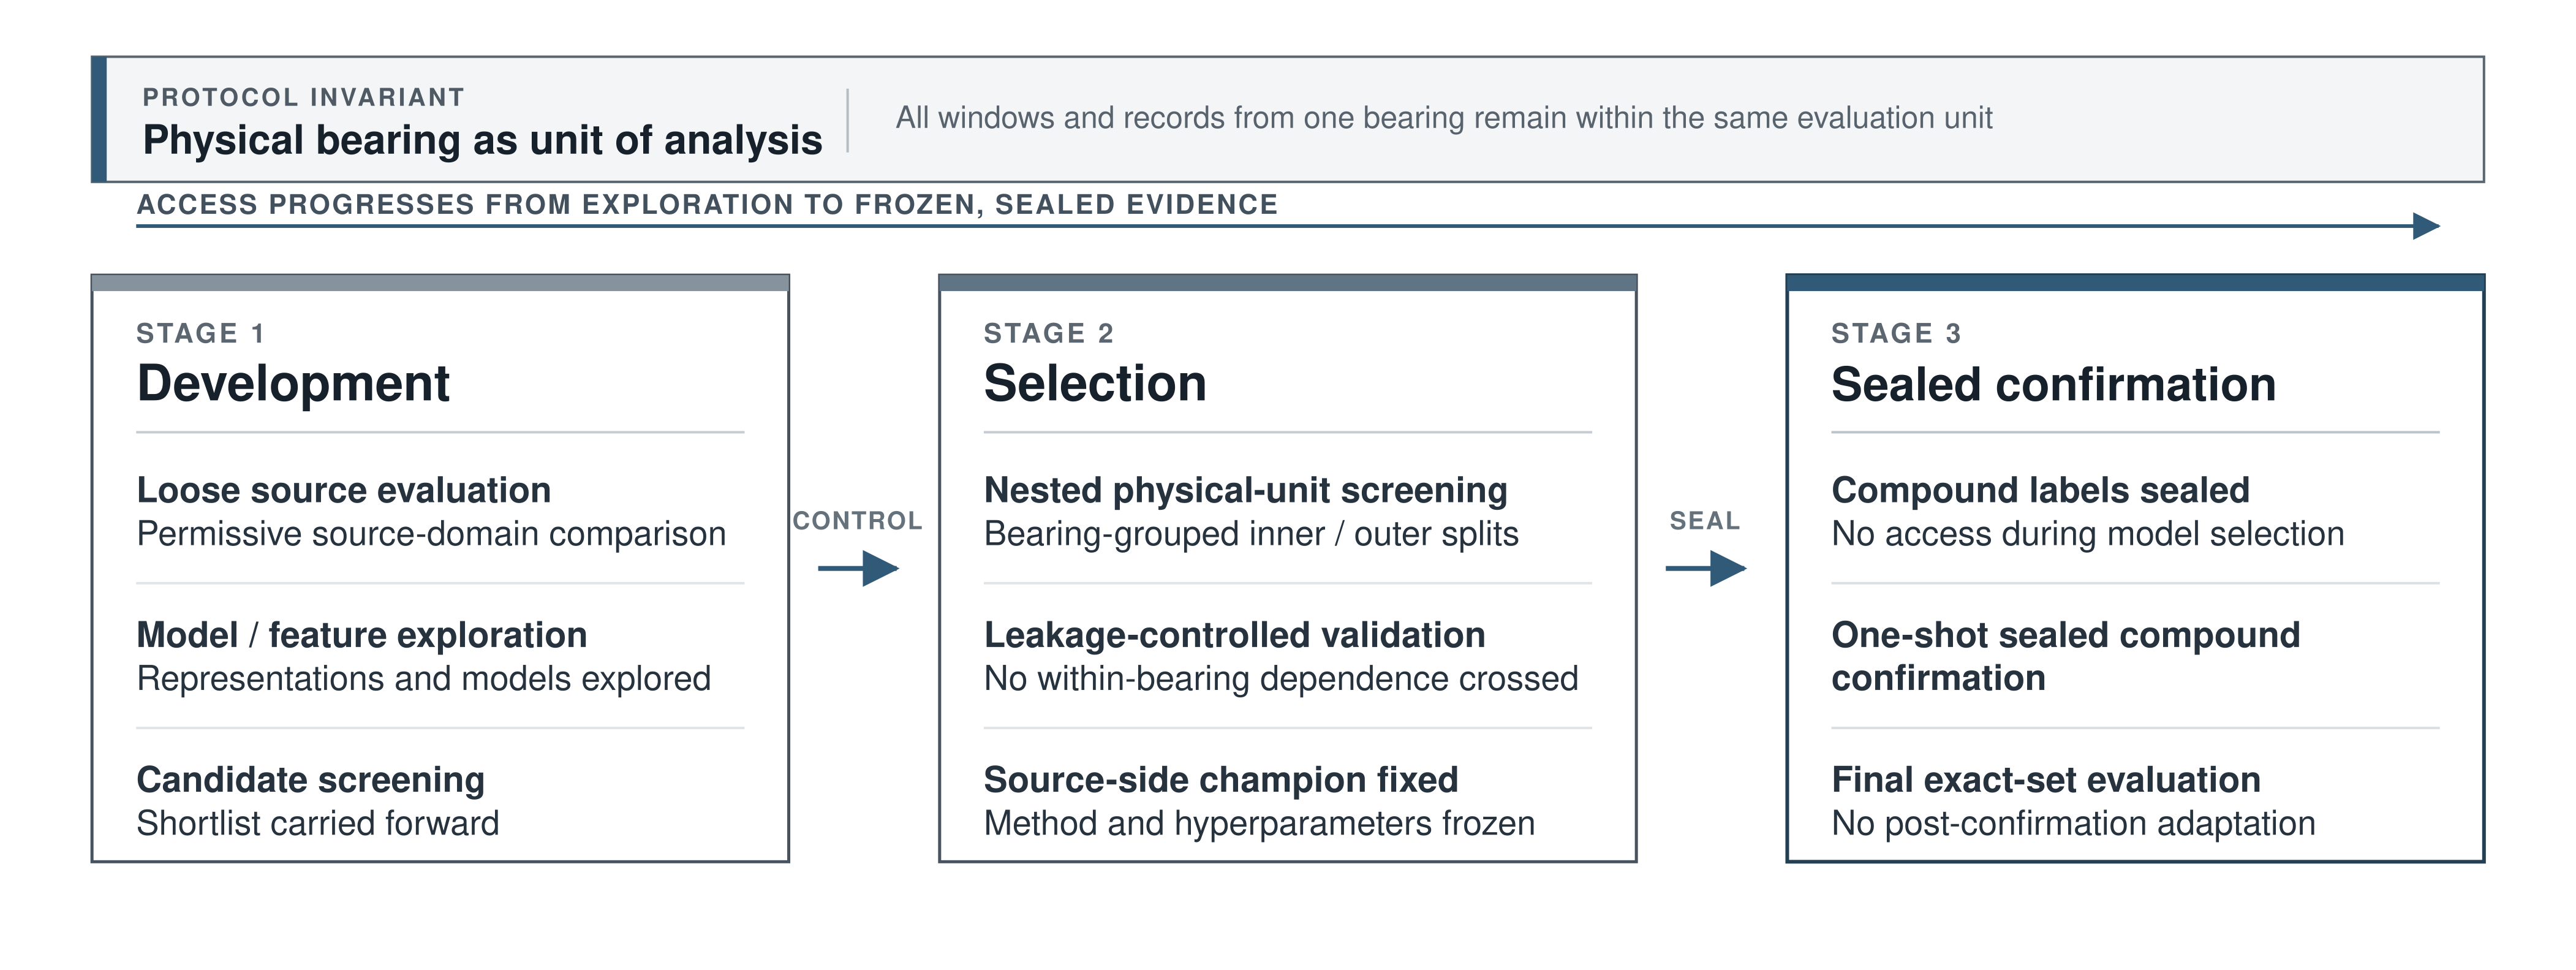
\includegraphics[width=\textwidth]{scgp_access_ladder_600dpi.png}
\caption{The SCGP access ladder. Evaluation progresses from exploratory source-domain development, through leakage-controlled physical-unit selection, to one-shot sealed compound confirmation. The physical bearing remains the invariant unit of analysis throughout: all windows and records derived from one bearing remain within the same evaluation partition.}
\label{fig:scgp_access_ladder}
\end{figure}

\section{Related Work}

Deep-learning research provides the immediate methodological background for machinery fault recognition. Reviews cover convolutional architectures, representation-learning pipelines, and the broader evolution of deep models for mechanical diagnosis \cite{r04,r06,r07}. Comparative studies further show that the reported score depends on both the representation and the learning model \cite{r05,r14}. Individual designs span direct deep pipelines, lightweight multiscale networks, improved convolutional models, motor-bearing classifiers, and hierarchical feature learners \cite{r08,r09,r10,r11,r12,r13}. Together, these studies establish a rich candidate space for fault recognition, but they do not by themselves determine whether the evaluation unit is independent or whether the final score supports a deployment claim.

Distribution shift has motivated transfer learning and domain adaptation across machines and operating conditions. Existing methods use cross-machine transfer, multilayer alignment, and benchmarked adaptation strategies to reduce differences between source and target distributions \cite{r03,r15,r16,r17,r18,r19}. Domain-generalization methods avoid direct target-domain tuning through contrastive learning, meta-learning, agent-based objectives, multisource formulations, and latent temporal models \cite{r20,r21,r22,r23,r24,r39}. Few-shot meta-learning and source-domain selection extend this landscape when target data are scarce or heterogeneous \cite{r36,r37,r38}. These approaches primarily change the representation, objective, or training distribution. They do not replace an evaluation contract that specifies which physical units remain independent, when model selection ends, and when target labels may be opened.

Evaluation dependence is a separate methodological problem. Leakage between vibration-signal partitions can inflate bearing-diagnosis results when related windows or records appear on both sides of a split \cite{r32}. Surveys of domain generalization likewise identify heterogeneity in datasets, domain definitions, and validation protocols as a barrier to comparing reported performance \cite{r33,r34}. A random window split can therefore measure recognition of repeated acquisition structure rather than transport to an unseen physical bearing. Even a group-level split does not fully resolve the problem if model selection, feature choice, or threshold tuning repeatedly uses the same groups that define the final endpoint. SCGP addresses this distinction by treating the physical bearing as the independent unit and by separating development, nested selection, and sealed confirmation.

Compound-fault diagnosis adds an output-level difficulty that is not captured by a component-wise metric. The operational question is often whether the complete set of damaged components has been recovered, not merely whether each component receives a favorable marginal score. Existing compound-diagnosis approaches include blind deconvolution, adaptive filtering with kernel learning, EEMD--CNN pipelines, recurrence analysis, and spatiotemporal decomposition \cite{r25,r26,r27,r28,r35}. These methods provide technical routes for extracting or classifying compound signatures, but their endpoint definitions and access permissions are not uniform. Reporting component discrimination together with exact-set recovery is therefore necessary to distinguish partial recognition from a correct compound decision.

Uncertainty-aware diagnosis provides a complementary perspective. Calibration, selective prediction, and Bayesian or risk-controlled uncertainty methods can improve interpretation of confidence after an evaluation population has been defined \cite{r29,r30,r31,r40}. However, confidence calibration cannot remove dependence between training and test records, undo label look-ahead, or establish that a selected model transports to a new bearing. Likewise, a stable confidence score does not imply stable model selection across physical-unit folds.

SCGP connects these research threads by making three boundaries explicit: the physical unit that must remain independent, the selection boundary at which the candidate configuration is frozen, and the compound-label opening that begins one-shot confirmation. Its purpose is not to replace existing classifiers or domain-generalization objectives, but to determine how much evidential status can be assigned to their scores under progressively stricter access states.

\section{Methods}

\subsection{Dataset, records, and independent units}

The HANOI HUST archive contains 99 MAT acquisitions from 33 physical bearings sampled at 51.2 kHz. The source partition contains 57 acquisitions from 19 bearings, with three load records per bearing. The sealed partition contains the remaining 42 acquisitions from 14 compound bearings. Source records represent the normal, inner-race, outer-race, and ball states used for development. The split was fixed before compound labels were opened, so confirmation records could not influence representation, hyperparameter, or threshold selection.

The physical bearing, rather than a waveform window or acquisition record, is the independent experimental unit. All load records and all derived windows from a bearing receive the same group identifier. Consequently, a held-out bearing contributes no waveform segment to its corresponding training fold. The design addresses two dependence structures that would otherwise be easy to overlook: repeated measurements of the same hardware and multiple deterministic windows extracted from the same acquisition.

Each waveform is converted into record-level features through a frozen windowing procedure. One-second windows contain 51,200 samples. Three extraction passes begin at offsets of 0, 0.25, and 0.5 s, with non-overlapping windows within each pass. Features are computed for each technical window and summarized by their componentwise median and interquartile range. This aggregation retains persistent spectral behavior while reducing the influence of isolated transients. The learning algorithms therefore operate on acquisition records, while inferential resampling remains at the bearing level.

The released source-window cache contains 1541 windows from the 57 source acquisitions and 19 source bearings. The three offsets correspond to sample positions 0, 12,800, and 25,600 at 51.2 kHz. The cache records the source archive hash, window shape, bearing identifier, acquisition identifier, and feature-construction provenance; the compound numeric files are not opened during source development. These metadata fields permit an independent audit of the split before any model is fitted.

\subsection{Problem formulation and access states}

We study compound fault recognition under three access states. Development permits source data for model and representation comparison. Selection fixes the candidate and hyperparameters through a nested physical-unit procedure. Confirmation keeps compound labels sealed until one-shot evaluation and prohibits post-opening tuning. The access contract, rather than only the code, is therefore frozen.

External resources follow their registered access states rather than being merged into one score. Mendeley Pump uses one workbook per factorial state \cite{r41}. Zenodo uses a balanced 320-record mixture from one rig across four speeds \cite{r42}. Both serve as quantitative boundary checks, not population-level replications. A Paderborn one-shot lockbox uses three physical bearing codes (K001, KA01, and KI01) and is reported separately because its rig, bearing type, sampling interface, and damage construction differ from HANOI HUST \cite{r43}.

For Paderborn, the frozen evaluation contains 240 records nested within three registered bearing codes. The healthy code and the two damaged codes were retained as a small cross-rig boundary sample; the frozen source configuration, feature representation, threshold, and prediction procedure were fixed before the component labels were opened. No Paderborn record was used for representation choice, hyperparameter tuning, threshold selection, or post-confirmation retraining; the effective independent unit is the bearing code.

\subsection{SCGP protocol}

SCGP comprises five variants. P0 and P1 use window- and record-random splits, P2 groups by physical unit, P3 nests model selection, and P4 seals compound labels until confirmation. \tbl{\ref{tab:scgp-contract}} defines their permissions. Results from different states are not interchangeable.

\begin{table*}[t]
\centering
\scriptsize
\setlength{\tabcolsep}{2pt}
\renewcommand{\arraystretch}{1.15}
\caption{SCGP access contract. States are defined before source or compound results are interpreted.}
\label{tab:scgp-contract}
\begin{tabular}{p{0.16\linewidth} p{0.23\linewidth} p{0.15\linewidth} p{0.18\linewidth} p{0.20\linewidth}}
\hline
State & Partition rule & Unit of analysis & Label access & Role in the analysis \\
\hline
P0 & Window-random split & Window & Open & Loose baseline that may leak bearing-level dependence \\
P1 & Record-random split & Record & Open & Common loose evaluation that still allows within-bearing coupling \\
P2 & Physical-unit group split & Bearing & Open & Leakage-controlled source-side comparison \\
P3 & Nested physical-unit selection & Bearing & Open during selection, frozen before confirmation & Selection state used to fix the source reference \\
P4 & Sealed compound confirmation & Bearing & Sealed until one-shot confirmation & Final confirmation state for compound recovery and boundary checks \\
\hline
\end{tabular}
\end{table*}

Operationally, SCGP is an access-controlled procedure. Let $D_s=\{(x_i,y_i,g_i)\}$ denote the source records, where $g_i$ is the physical-bearing identifier, let $\mathcal{C}$ be the registered candidate set, and let $D_c$ denote the confirmation records whose compound labels are unavailable during development. For each outer split, SCGP (i) partitions $D_s$ by the declared unit, (ii) fits every representation and candidate using only the permitted inner-training records, (iii) selects $c^\ast$ with the prespecified endpoint, (iv) refits $c^\ast$ on the allowed development records, and (v) evaluates it once on the untouched outer records. For P4, the frozen $c^\ast$, representation, preprocessing parameters, and threshold are copied unchanged to $D_c$; compound labels are opened only after predictions and audit hashes have been written. No confirmation result can therefore change $c^\ast$, the feature map, or the threshold. The procedure outputs the split manifest, selected candidate, predictions, unit-level metrics, and an access log. This explicit state transition distinguishes SCGP from an ordinary held-out test in which the timing and permissions of selection and label opening are often left implicit.

The relationship between SCGP and commonly used evaluation practices is summarized in \tbl{\ref{tab:scgp-positioning}}.

\begin{table*}[t]
\centering
\scriptsize
\setlength{\tabcolsep}{3pt}
\caption{Positioning SCGP relative to commonly used evaluation practices. The added contribution is an explicit, auditable contract linking physical-unit identity, selection permissions, compound-label opening, and joint endpoints; the individual ingredients are not claimed as new algorithms.}
\label{tab:scgp-positioning}
\begin{tabular}{p{0.22\linewidth}p{0.30\linewidth}p{0.38\linewidth}}
\hline
Existing practice & Typical guarantee & SCGP-specific operational addition \\
\hline
Grouped cross-validation & Reduces same-group leakage & Declares the physical bearing as the independent unit and records its split manifest and aggregation unit \\
Nested cross-validation & Separates tuning from outer evaluation & Freezes the candidate, preprocessing, threshold, and selection permission at an explicit access boundary \\
Locked or held-out test set & Protects a final score from tuning & Seals compound labels until predictions and audit hashes are written, with one-shot opening recorded \\
Multilabel metrics & Reports component or set performance & Requires component-level and exact-set endpoints at the same declared unit, with per-unit uncertainty \\
\hline
\end{tabular}
\end{table*}

\subsection{Representations and baselines}

The frozen representation family contains robust time statistics, fixed physical-frequency log-power bands, and envelope log-power bands. The statistics block includes the mean, standard deviation, root-mean-square value, absolute mean, extrema, and peak-to-peak range. It also includes skewness, excess kurtosis, crest factor, impulse factor, shape factor, and an envelope-based peak factor. Median and interquartile-range aggregation produces 28 values per extraction offset and 84 values after concatenating the three offsets.

The two spectral views use the same frequency partition, isolating representation rather than dimensionality. After mean removal and Hann tapering, squared real-Fourier magnitudes are summed within 64 equal-width bands from 0 to 25.6 kHz. A base-10 logarithm is applied after a fixed numerical floor. The envelope view computes the analytic-signal magnitude with the Hilbert transform and removes its mean. It then applies the same taper, transform, band integration, and logarithm. Median--interquartile aggregation yields 128 values per offset and 384 values for either spectral view. The combined \texttt{all} representation concatenates all three blocks.

The prediction target is a three-component vector for inner-race, outer-race, and ball faults. A separate binary estimator produces the positive-class probability for each component, and a fixed threshold of 0.5 converts each probability into a component decision. The threshold was fixed before compound confirmation to prevent target-label calibration and is therefore a prespecified operating convention rather than a claim of optimality. Exact-set correctness requires all three component decisions to match simultaneously. Thresholds are not optimized on the compound partition; threshold sensitivity is treated as an operating-boundary analysis rather than as an additional selection step.

The source-selected, subsequently frozen reference is an L2-regularized logistic model using \texttt{envelope\_log\_power}. Features are standardized within each training fold, class weights are balanced, $C=10$, and optimization is capped at 5000 iterations. The selection rule was registered before the final source comparison; the model identity was frozen only after that source-side comparison. The frozen comparison also includes logistic models, linear and radial-basis SVMs, random forests, extremely randomized trees, an empirical-prior control, multilayer perceptrons, and the implemented NOACE variants. Compact tree and kernel grids test protocol sensitivity across different decision rules without unrestricted hyperparameter search. A separately registered G3 audit adds Random Forest, source-only GroupDRO-style logistic reweighting, MiniROCKET, WDCNN, ResNet1D, and InceptionTime-style comparators. G3 models are evaluated only on the bearing-grouped outer protocol and are not allowed to alter the primary model choice.

The comparator set is layered by evidential role. The source reference and representation ablation define the prespecified internal comparison. Classical alternatives test whether the selected row depends on an unusually weak baseline. Modern alternatives examine whether the protocol-dependent pattern remains after stronger candidates are introduced. Sealed-confirmation models are reported separately because they answer a different question from source-side selection.

Here, NOACE denotes the implemented nuisance-residualized compositional-evidence baseline; ``orthogonal'' refers only to numerical orthogonality to the fitted training design, not to causal nuisance removal. The implementation and ablation artifact are versioned with the submission package.

Within each training fold, a linear nuisance model regresses the feature vector on one-hot bearing-type and load indicators. The residual is used for subsequent fitting, and nuisance coefficients and category levels are frozen before test prediction. If a deployment bearing type is absent from the training categories, the current implementation raises an explicit error rather than silently extrapolating; bearing type is therefore treated as available metadata, not as a universally available sensor measurement.

Let $\mu_{\emptyset}$ be the healthy residual mean and $\mu_j$ the singleton mean for component $j\in\{1,2,3\}$. For subset $S$, the additive prototype is $\mu_S=\mu_{\emptyset}+\sum_{j\in S}(\mu_j-\mu_{\emptyset})$. With diagonal residual variance $v_k$ and subset prototype $\mu_S$, a record with residual feature vector $r$ receives subset energy $E_S(r)=\frac{1}{2}\sum_k (r_k-\mu_{S,k})^2/v_k$. Subset weights are proportional to $\exp[-E_S(r)/T]$ with fixed temperature $T=1$ and equal subset priors; component probabilities are obtained by marginalizing subset indicators. The registered ablations vary residualization, additive prototypes, subset prior, temperature, and diagonal versus pooled variance.

The supplementary physics-feature variant resamples the fixed and envelope log-power spectra to an order axis using recorded shaft speed in revolutions per minute. The frequency axis is linearly interpolated to 64 order bins spanning 0.5--256 orders; missing or non-positive speed produces an all-zero 64-bin view. In the 57-record HANOI source cache, speed was available for 24 records and missing for 33; no separate missingness mask was appended. This zero-fill convention is therefore a strong comparator assumption and was not used to support the primary SCGP claim. The same procedure is applied to the HANOI source cache within each fold; it is not asserted to be physically identical across Paderborn or other rigs. The variant is a comparator, not the main method. It is distinct from the separately implemented MLP comparator, identified as \texttt{mlp\_deep} in the machine-readable artifact.

The exact candidate identifiers, parameter values, split manifests, and prediction targets are serialized in the machine-readable result files supplied with the submission package. The primary logistic reference is fixed at $C=10$; the remaining classical candidates use the registered compact grids rather than an unrestricted search. G3 comparators use the same bearing-grouped outer splits, physical-bearing aggregation, and I0 source-only information budget, so their audit cannot retroactively change the primary model choice.

\subsection{Implementation and reproducibility}

The analysis was executed with Python 3.11. The environment specification uses PyTorch 2.6, torchvision 0.21, torchaudio 2.6, and CUDA 12.4 for waveform models, together with NumPy, SciPy, pandas, and scikit-learn for feature processing and classical models. The recorded execution environment reports NumPy 2.3.5, SciPy 1.16.3, and scikit-learn 1.8.0 for the corresponding audit artifacts. Classical models were evaluated on the frozen feature caches; neural baselines used the recorded GPU implementation and fixed downsampling/training budgets. Source builders, split manifests, archive hashes, and audit JSON files are included in the reproducibility package. The crossed endpoint audit additionally includes the three \texttt{record\_predictions.npz} files, \texttt{factorial\_endpoint\_metrics.json}, \texttt{hanoi\_hust\_noace\_ablation.json}, and the executable ablation script.

Randomness is separated by role. The frozen HANOI confirmation uses the registered random state 20260727, the primary bearing-cluster bootstrap uses seed 20260728 with 10,000 resamples, and the source stability audit repeats the fixed protocol with seeds 42, 7, 21, 84, and 168. These repeated runs do not redefine the endpoint or replace the prespecified primary result. Every prediction file is linked to its split manifest, model family, representation, seed, and source-code provenance.

\subsection{Metrics and inference}

We report component- and set-level metrics because one accuracy value cannot characterize compound recognition. Component metrics are AUROC, balanced accuracy, AUPR, Brier score, and macro-F1. Set metrics are exact-set accuracy and Hamming loss. Boundary analyses also report calibration error, selective accuracy, risk--coverage behavior, and efficiency.

Let $\mathbf{y}_i\in\{0,1\}^{3}$ denote the true component vector for record $i$, $\hat{\mathbf{y}}_i$ the thresholded prediction, and $\mathbf{p}_i$ the corresponding probability vector. Exact-set accuracy is
\[
\frac{1}{n}\sum_{i=1}^{n}\mathbb{I}\!\left(\mathbf{y}_i=\hat{\mathbf{y}}_i\right),
\]
whereas Hamming loss averages disagreements over the $3n$ binary decisions. Component metrics are calculated separately for the three faults and then averaged. Favorable marginal rankings can therefore coexist with an incorrect joint label set.

The unit of each reported endpoint is explicit. G2 record-grouped values are calculated after window-to-record aggregation, with each acquisition record contributing one prediction; G2 bearing-grouped values first average the three load-record probabilities within each physical bearing and then calculate the metrics over bearings. G3 and the legacy NOACE comparisons are bearing-level endpoints after the same load aggregation. Exact-set accuracy always uses the joint three-component vector at the stated endpoint unit, and all confidence intervals resample physical bearings rather than records or windows. Numerators and denominators are therefore determined by the declared access state, not by the number of derived windows. The crossed audit stores pre-aggregation record predictions for the fixed record-grouped, fixed bearing-grouped, and nested bearing-grouped cells, together with post-aggregation arrays, split manifests, and the aggregation script. For the two fixed cells, endpoint summaries use identical fitted-model outputs, preprocessing, class weighting, and threshold 0.5; the nested cell instead uses the candidate selected within each outer fold. Within any cell, only prediction-stage aggregation and endpoint metric unit differ.

For the nested cell, model identity is fold-specific rather than frozen globally. Inner selection is completed before outer-test prediction; one selected candidate is refit per outer fold, and that same candidate generates all test-record probabilities for the fold. Bearing aggregation is then a deterministic mean of the three load probabilities from that selected candidate. No probabilities from different candidates are mixed, and the component threshold remains 0.5 for every candidate.

Calibration is evaluated at both component and set levels. Component expected calibration error compares predicted probabilities with empirical binary outcomes within confidence bins. Set confidence is the model-implied confidence assigned to the complete thresholded vector, and set-level calibration error compares that confidence with exact-set correctness. Selective prediction sorts records by set confidence and reports exact-set accuracy as coverage is reduced. The area under the resulting risk--coverage curve summarizes the trade-off but does not replace the individual coverage points, because a non-monotonic curve can reveal high-confidence failure groups.

Comparisons are made at the physical-bearing level. Percentile 95\% confidence intervals use 10,000 bearing-cluster bootstrap resamples (seed 20260728). The registered paired comparator tests use exact-set correctness only: each bearing contributes one paired value after its three load probabilities have been averaged, so the values are binary (0 or 1). Because the support is discrete and ties are frequent, the Wilcoxon signed-rank calculation is retained only as a supplementary descriptive check; the main evidence is the per-bearing difference, its cluster-bootstrap interval, and the complete per-bearing outcome table in the audit artifact. Individual windows are never treated as independent inferential units. The 100 G3 outer splits are correlated repeated resamples of the same 19 bearings; split-level sign-permutation values are consequently reported as conditional resampling summaries, not as evidence from 100 independent experiments. Bearing-level bootstrap intervals and per-bearing outcomes determine the inferential unit.

Outer-fold selection frequencies characterize stability without combining access states into a common leaderboard. They show whether one family--representation configuration is repeatedly preferred under the nested procedure.

\section{Results}

For transparency, two frozen analysis generations are retained. The legacy source/NOACE tables and figures below reproduce the earlier 19-bearing audit (record-level model comparison and its sealed confirmation); they are preserved for traceability and are not the primary headline estimate. The primary matched-protocol estimate is the new 2$\times$2 endpoint audit. For a metric $m_s$ in split $s$, the point estimate is the registered repeated-split mean $\bar m=S^{-1}\sum_{s=1}^{S}m_s$; the displayed prediction counts are descriptive repeated-split counts, not independent-sample proportions. Exact-set intervals are 19-bearing cluster-bootstrap intervals computed from per-bearing mean outcomes, conditional on the registered repeated-split procedure. Record-grouped splitting gives record-level AUROC/exact-set 0.951/0.776 (exact-set 1086/1400, CI 0.626--0.899; AUROC CI 0.864--0.987) and bearing-aggregated 0.959/0.791 (866/1093, CI 0.635--0.919; AUROC CI 0.884--0.993); fixed bearing-grouped splitting gives 0.828/0.510 (765/1500, CI 0.417--0.747; AUROC CI 0.629--0.902) and 0.860/0.490 (245/500, CI 0.400--0.776; AUROC CI 0.656--0.927), respectively; nested bearing-level selection gives 0.777/0.420 (630/1500, CI 0.345--0.686; AUROC CI 0.559--0.846) and 0.803/0.406 (203/500, CI 0.328--0.701; AUROC CI 0.567--0.850). These cells are reported separately and are never pooled.

\subsection{The primary result is a crossed partition--aggregation analysis}

The crossed audit used the same frozen logistic--envelope reference for the two fixed cells and retained both pre-aggregation record predictions and post-aggregation bearing predictions. Under record-grouped splitting, the fixed reference gave record-level AUROC 0.951 and exact-set accuracy 0.776, whereas bearing aggregation yielded 0.959 and 0.791. Under fixed bearing-grouped splitting, the corresponding values were 0.828/0.510 and 0.860/0.490. The nested cell is different: each outer bearing split performed registered inner model selection, refit the selected candidate on that fold's allowed training records, predicted all three load records with that one selected candidate, and only then produced record-level and bearing-aggregated endpoints. Its values were 0.777/0.420 and 0.803/0.406. The 100 nested outer folds selected logistic--envelope configurations 54 times, extra-trees--envelope configurations 29 times, and RBF-SVM--envelope configurations 17 times (all candidates used the registered envelope view); the exact hyperparameter frequencies are in the split manifest. Thus the nested values are not fixed-reference estimates. The crossed result separates fixed-reference endpoint contrasts from nested-selection transport and does not assign the entire decline to physical-unit separation alone.

The fixed record-grouped endpoint is the most permissive source reference; fixed bearing-grouped evaluation measures transport to unseen physical units with the candidate frozen; nested bearing-grouped evaluation measures transport after model selection is included in the outer boundary. We therefore report them as separate access states rather than as one averaged score. The remainder of the Results section explains the source audit, selection instability, model-family robustness, sealed confirmation, and operating boundaries that qualify these endpoints.

\subsection{Secondary legacy audit: conditional source reference}

On the 19-bearing source partition, the prespecified mean component AUROC endpoint selected \texttt{logistic\_l2 + envelope\_log\_power} (AUROC, 0.814). Its balanced accuracy was 0.743, AUPR 0.661, Brier score 0.161, macro-F1 0.743, exact-set accuracy 0.544, and Hamming loss 0.199.

\tbl{\ref{tab:hanoi_main_results}} compares the source reference with the principal alternatives.

The endpoint differences from the selected representation are reported in \tbl{\ref{tab:hanoi_view_ablation}} in Section~4.5, and \fig{\ref{fig:source_champion}} summarizes the source ranking and representation trade-offs.

\begin{table*}[t]
\centering
\footnotesize
\setlength{\tabcolsep}{3pt}
\renewcommand{\arraystretch}{1.12}
\caption{Legacy frozen source comparison on the 19-bearing HANOI HUST partition. These values are retained for audit traceability; the primary matched G2/G3 estimates are reported separately in the manuscript.}
\label{tab:hanoi_main_results}
\resizebox{\textwidth}{!}{%
\begin{tabular}{llrrrrrrr}
\toprule
Method & Representation & AUROC & BAcc & AUPR & Brier & Macro-F1 & Exact-set & Hamming \\
\midrule
\texttt{logistic\_l2} & \texttt{envelope\_log\_power} & 0.814 & 0.743 & 0.661 & 0.161 & 0.743 & 0.544 & 0.199 \\
\texttt{logistic\_l2} & \texttt{all} & 0.807 & 0.729 & 0.651 & 0.141 & 0.728 & 0.596 & 0.199 \\
\texttt{logistic\_l2} & \texttt{fixed\_log\_power} & 0.753 & 0.677 & 0.610 & 0.169 & 0.670 & 0.404 & 0.275 \\
\texttt{logistic\_l2} & \texttt{statistics} & 0.721 & 0.729 & 0.589 & 0.198 & 0.722 & 0.544 & 0.216 \\
\texttt{extra\_trees} & \texttt{envelope\_log\_power} & 0.747 & 0.658 & 0.536 & 0.172 & 0.656 & 0.596 & 0.251 \\
\texttt{rbf\_svm} & \texttt{all} & 0.725 & 0.612 & 0.581 & 0.160 & 0.630 & 0.474 & 0.228 \\
\texttt{empirical\_prior} & \texttt{statistics} & 0.000 & 0.500 & 0.246 & 0.206 & 0.430 & 0.263 & 0.246 \\
\bottomrule
\end{tabular}
}
\vspace{0.4em}
\par\small\noindent
Repeated frozen runs produced the same selected row. Bearing-level uncertainty and paired exact-set comparisons are reported in Supplementary Table~S4.
\end{table*}


\clearpage

\begin{figure*}[!t]
\centering
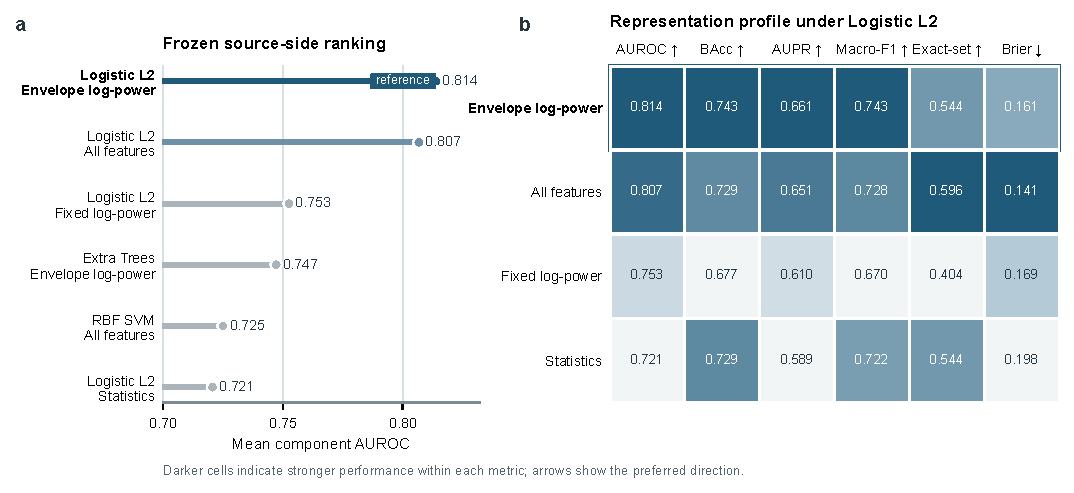
\includegraphics[width=\textwidth]{figures/figure2_source_champion.pdf}
\caption{Legacy frozen source reference and representation profile. (a) Six model--representation pairs ranked by mean component AUROC on 19 source bearings. (b) Four representations compared with \texttt{logistic\_l2}; darker cells denote better performance after reversing the Brier-score direction. \texttt{envelope\_log\_power} leads component discrimination, whereas \texttt{all} has higher exact-set accuracy and a lower Brier score. Values are point estimates from the legacy audit; the matched G2/G3 estimates are reported separately.}
\label{fig:source_champion}
\end{figure*}

\subsection{Secondary legacy audit: repeatability and negative controls}

All five registered seeds (42, 7, 21, 84, and 168) selected \texttt{logistic\_l2 + envelope\_log\_power} and produced identical aggregate results. Given deterministic folds and a convex estimator, this repeatability rules out favorable stochastic initialization as the explanation for the source row.

Label shuffling provided a stronger negative control. Across five seeds, mean component AUROC ranged from 0.325 to 0.565 and exact-set accuracy from 0.175 to 0.316. Both were below the observed values of 0.814 and 0.544. Disrupting the feature--label mapping therefore degraded both endpoints but did not test whether the remaining associations were causal.

Identity probes separated fault information from two nuisance variables. Bearing type remained predictable under load-held-out evaluation (balanced accuracy, 0.872). Load prediction under bearing-held-out evaluation was near chance (balanced accuracy, 0.281). The bearing-type signal supports bearing-level grouping, whereas load identity alone is unlikely to explain the source ranking.

The source cross-distribution audit found five bearing-type codes (4--8). Type 4 contained no ball-state record, whereas types 5--8 each contained normal, inner-race, outer-race, and ball records across the three loads. Thus, bearing-level grouping prevents same-bearing leakage but does not remove hardware-type/label confounding; a leave-type-out experiment would be required for that stronger claim.

\subsection{Sealed compound boundary confirmation}

We evaluated 14 compound bearings under sealed compound boundary confirmation. After averaging the three load probabilities within each bearing, the legacy sealed-confirmation model, \texttt{noace\_classical}, achieved mean component AUROC 0.621 (95\% bearing-cluster bootstrap interval, 0.496--0.739) and exact-set accuracy 0/14 (interval, 0--0). On the same partition, \texttt{source\_logistic\_l2} achieved AUROC 0.811 (0.668--0.923) and exact-set accuracy 2/14 = 0.143 (0--0.357). The MLP comparator (artifact key \texttt{mlp\_deep}) reached AUROC 0.881 (0.706--1.000) but exact-set accuracy 0/14 (0--0). Per-bearing outcomes are provided in the sealed uncertainty audit; all intervals are conditional on this 14-bearing lockbox.

\subsection{Secondary Paderborn sealed compound boundary check}

The Mendeley Pump and Zenodo workbook-level analyses use different tasks and algorithms and are retained in Supplementary Information rather than used as primary evidence. Their separate transductive workbook-level method, safe-reference definition, and label-access audit are documented only in the supplementary files; none is treated as HANOI's logistic, NOACE, or G3 implementation.

The Paderborn one-shot lockbox contained 240 records from three physical bearing codes. The frozen HANOI source reference correctly identified the healthy code but failed to recover the inner- and outer-race labels: component AUROC was 0.000 for both observed components and exact-set accuracy was 1/3 at the bearing-code level. The effective independent unit is therefore three codes, not 240 records. The lockbox was evaluated once and was not used for pooled replication or external tuning.

The legacy endpoint differences are summarized in \tbl{\ref{tab:hanoi_view_ablation}}, while the quantitative sealed-compound and external confirmation tracks are summarized in \tbl{\ref{tab:hanoi_boundary_results}}. \fig{\ref{fig:sealed_confirmation_gap}} contrasts component and exact-set endpoints on HANOI HUST.

\begin{table}[t]
\centering
\footnotesize
\setlength{\tabcolsep}{5pt}
\renewcommand{\arraystretch}{1.10}
\caption{Legacy endpoint differences from the AUROC-selected source representation under \texttt{logistic\_l2}.}
\label{tab:hanoi_view_ablation}
\begin{tabular}{lrrrr}
\toprule
View & $C$ & $\Delta$ AUROC & $\Delta$ Exact-set & $\Delta$ Brier \\
\midrule
\texttt{envelope\_log\_power} & 10.00 & 0.000 & 0.000 & 0.000 \\
\texttt{all} & 0.10 & $-0.007$ & $+0.053$ & $-0.020$ \\
\texttt{fixed\_log\_power} & 0.01 & $-0.061$ & $-0.140$ & $+0.008$ \\
\texttt{statistics} & 10.00 & $-0.093$ & 0.000 & $+0.038$ \\
\bottomrule
\end{tabular}
\vspace{0.4em}
\par\small\noindent
Each $\Delta$ is the view minus \texttt{envelope\_log\_power}; lower Brier score is better. Table~\ref{tab:hanoi_main_results} reports the full point estimates.
\end{table}

\begin{table*}[t]
\centering
\footnotesize
\setlength{\tabcolsep}{4pt}
\renewcommand{\arraystretch}{1.10}
\caption{Documented HANOI HUST held-out confirmation and Paderborn cross-rig boundary checks.}
\label{tab:hanoi_boundary_results}
\begin{tabular}{p{0.13\textwidth}p{0.17\textwidth}p{0.27\textwidth}p{0.35\textwidth}}
\toprule
Resource & Evaluation unit & Observed result & Evidential interpretation \\
\midrule
HANOI HUST & 14 held-out compound bearings & Across three models, component AUROC was 0.621--0.881 and exact-set accuracy was 0--0.143. & Historical held-out confirmation under a documented local freeze. \\
Paderborn pilot & 3 physical bearing codes (240 records) & Inner-/outer-race AUROC was 0.000/0.000; exact-set accuracy was 1/3, with only the healthy code recovered. & Frozen one-shot score; negative pilot evidence from three independent codes. \\
Paderborn extension & 12 new physical bearing codes (960 records) & Inner-/outer-race AUROC was 0.344/0.719; exact-set accuracy was 3/12 (95\% exact CI, 0.055--0.572). & Pre-access-frozen, disjoint external score without Paderborn tuning across 12 new codes. \\
\bottomrule
\end{tabular}
\vspace{0.4em}
\par\small\noindent
Mendeley Pump and Zenodo single-rig checks are reported in Supplementary Information at their native tasks and evaluation units.
\end{table*}


\begin{figure}[!t]
\centering
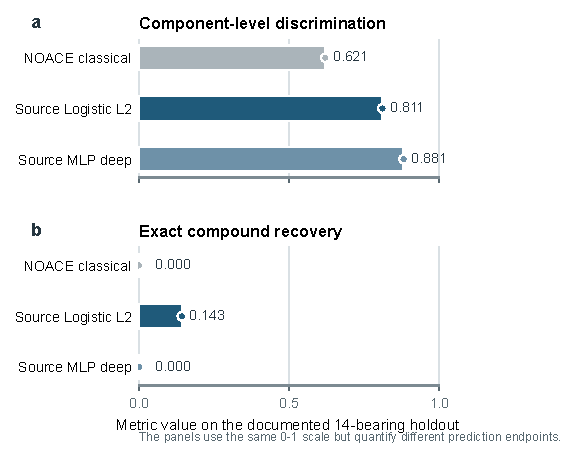
\includegraphics[width=\columnwidth]{figures/figure3_sealed_confirmation_gap.pdf}
\caption{Sealed confirmation on 14 compound bearings. (a) Mean component AUROC and (b) exact-set accuracy for three models. Both panels use a 0--1 scale but represent different endpoints and are not directly subtractable. Bars are point estimates; the small 14-bearing lockbox produces wide discrete cluster-bootstrap intervals, which are reported in the Results text and audit file rather than overlaid on the compact plot. Component AUROC ranges from 0.621 to 0.881, whereas exact-set accuracy ranges from 0 to 0.143.}
\label{fig:sealed_confirmation_gap}
\end{figure}

\subsection{Secondary legacy audit: 19-fold protocol tightening}

The stricter nested physical-unit screen achieved mean component AUROC 0.701, balanced accuracy 0.685, exact-set accuracy 0.526, and Brier score 0.169. Relative to frozen source evaluation, AUROC decreased by 0.112, balanced accuracy by 0.058, and exact-set accuracy by 0.018. These changes describe the registered state-specific procedure; because candidate pools and endpoint targets differ, they are not a clean estimator of selection alone.


Endpoint choice also changed the preferred configuration. \texttt{rf + statistics} reached exact-set accuracy 0.579, while \texttt{extra\_trees + envelope\_log\_power} reached 0.544. Both \texttt{linear\_svm + envelope\_log\_power} and \texttt{rbf\_svm + all} had lower mean component AUROC than the source reference.

Across 19 leave-one-bearing-out folds, \texttt{logistic\_l2 + all} accounted for 10 selections after pooling hyperparameters. \texttt{logistic\_l2 + statistics} accounted for four, the two \texttt{extra\_trees} views for four, and \texttt{logistic\_l2 + fixed\_log\_power} for one. The nested procedure therefore did not select one invariant configuration.

This 19-fold histogram belongs to the legacy audit and uses a different candidate pool and endpoint from the primary 100-fold nested audit above. It demonstrates instability within that legacy state-specific procedure, not a comparison with the primary 54/29/17 selection counts, a universal ranking reversal, or a general theorem about nested selection.

\subsection{Source-only robustness audit across model families}

To test whether the bearing-grouped result depended on one particular estimator, we registered a separate G3 audit before reading any external waveform. Every candidate used the same 100 bearing-grouped outer splits, the same physical-bearing aggregation, and the I0 source-only information budget. The fixed logistic reference was compared with six comparator families: random forest, GroupDRO-style logistic regression, MiniROCKET, WDCNN, ResNet1D, and InceptionTime. Their architecture, downsampling, training budget, and negative results were retained in the artifact manifest. This audit changes the estimator at one fixed bearing-grouped endpoint; it is not evidence that every possible partition--aggregation contrast is estimator-invariant.

\begin{table*}[t]
\centering
\footnotesize
\setlength{\tabcolsep}{5pt}
\renewcommand{\arraystretch}{1.12}
\caption{Source-only G3 robustness audit under the identical 100 bearing-grouped outer splits. All scores are computed after aggregation to the physical-bearing unit. The raw-waveform models use a fixed downsampling factor of 64 and are reported as diagnostic R2 implementations; no model was tuned on the outer test bearings.}
\label{tab:g3-audit}
\begin{tabular}{l l r r r r r}
\toprule
Method & Input / budget & AUROC & AUPR & Bal. Acc. & Macro-F1 & Exact set \\
\midrule
Fixed logistic & Envelope features / I0 & 0.860 & 0.843 & 0.712 & 0.675 & 0.490 \\
Random forest & Envelope features / I0 & 0.785 & 0.750 & 0.666 & 0.628 & 0.458 \\
GroupDRO-style logistic & Envelope features / I0 & 0.845 & 0.825 & 0.721 & 0.680 & 0.482 \\
MiniROCKET & Raw waveform / I0 & 0.751 & 0.708 & 0.682 & 0.628 & 0.556 \\
WDCNN-style & Raw waveform / I0 & 0.630 & 0.608 & 0.530 & 0.386 & 0.116 \\
ResNet1D & Raw waveform / I0 & 0.609 & 0.607 & 0.521 & 0.373 & 0.120 \\
InceptionTime-style & Raw waveform / I0 & 0.569 & 0.565 & 0.516 & 0.370 & 0.120 \\
\bottomrule
\end{tabular}
\end{table*}


\tbl{\ref{tab:g3-audit}} shows that the fixed logistic reference had the highest point estimate for component discrimination among the evaluated implementations at this bearing-grouped endpoint. GroupDRO was close in point estimate, with a 0.017 AUROC difference in the conditional split-level comparison; the split-level sign-permutation calculation is retained only in Supplementary Information because the 100 splits reuse the same 19 bearings. The raw-waveform implementations do not automatically improve transportability; MiniROCKET had the highest point estimate among them, while the three compact neural implementations were weaker. Exact-set accuracy also remains sensitive to the implementation and should not be inferred from AUROC alone. These results retain the engineered-feature logistic model as a conditional source reference while treating the family audit as an endpoint-specific supplementary analysis.

\fig{\ref{fig:protocol_sensitivity}} shows score changes and foldwise selection frequencies; \tbl{6} reports source-boundary statistics.

\begin{figure}[!t]
\centering
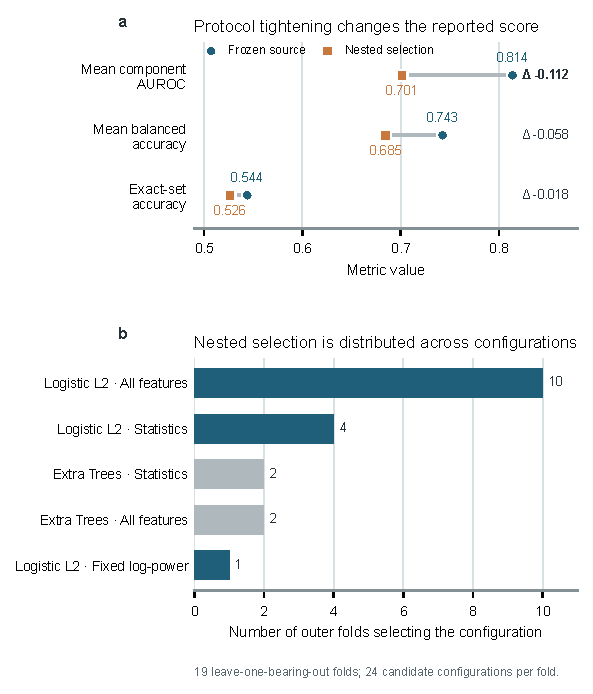
\includegraphics[width=\columnwidth]{figures/figure4_protocol_sensitivity.pdf}
\caption{Legacy protocol tightening and selection stability. (a) Frozen source and nested physical-unit point estimates for mean component AUROC, balanced accuracy, and exact-set accuracy on 19 source bearings. Lines show state-specific changes; distinct metrics are not averaged. (b) Family--representation selections across 19 outer folds after pooling hyperparameters. Each fold screens 24 configurations. Counts are selection frequencies, not uncertainty estimates, and candidate pools differ across access states.}
\label{fig:protocol_sensitivity}
\end{figure}

\input{HANOI_HUST_Table5_LaTeX_20260728.tex}

The source reference exact-set accuracy of 0.544 had a 95\% bearing-cluster bootstrap interval of 0.333--0.754. Relative to \texttt{NOACE-classical} and \texttt{NOACE-physics}, the paired difference was $-3.51$ percentage points (95\% CI, $-28.1$ to 21.1; Holm-adjusted $p=1.000$; $d_z=-0.061$). The difference from the MLP comparator was 0.00 percentage points (95\% CI, $-17.5$ to 15.8; Holm-adjusted $p=1.000$). Exact-set comparisons therefore did not support superiority over the NOACE-classical or MLP comparator families.

The registered NOACE ablation clarifies what the comparator does and does not establish. Across the same 19-bearing leave-one-bearing-out folds, the full residualized additive model reached AUROC 0.812 and exact-set accuracy 0.579 (19-bearing bootstrap 95\% CI, 0.368--0.789). Removing residualization increased these point estimates to 0.823 and 0.632 (CI, 0.421--0.842), so residualization was not supported as a beneficial design choice in this dataset. Replacing additive subset prototypes by a healthy-only prototype collapsed performance to AUROC 0.500 and exact-set accuracy 0 (CI, 0--0), while pooled rather than feature-wise variance reduced AUROC to 0.646 and exact-set accuracy to 0.474 (CI, 0.263--0.684). Temperature changes ($T=0.5$ and $T=2$) produced AUROC 0.805 and 0.807, respectively, with exact-set accuracy 0.579 (CI, 0.368--0.789); a source-frequency subset prior was unchanged at the displayed precision. Fold-wise residual--nuisance correlations were below $3.3\times10^{-15}$; this value is an algebraic consequence of least-squares residualization against the fitted training design, not independent evidence of nuisance removal. NOACE is therefore retained as a transparent comparator rather than as a validated nuisance-removal contribution.

\subsection{Calibration, robustness, and efficiency define the operating boundary}

Calibration revealed a failure mode that is hidden by aggregate AUROC. The set-level expected calibration error was 0.298 and the area under the risk--coverage curve was 0.309. Component calibration was heterogeneous: ECE was 0.169 for the inner-race component, 0.296 for the outer-race component, and 0.068 for the ball component. Thus, probability quality depended strongly on which constituent fault was being assessed.

The fixed-threshold operating audit showed that exact-set accuracy was not invariant to the component threshold. For the source reference, record-level exact-set accuracy ranged from 0.491 to 0.561 across thresholds 0.2--0.8, while bearing-level exact-set accuracy ranged from 0.474 to 0.579. This is a prespecified common-threshold scan performed after the frozen predictions were generated; it is not a post hoc choice of the best threshold. Component-specific thresholds and a joint exact-set-optimized threshold were not estimated because target-label tuning was prohibited. The pre-specified threshold 0.5 was retained for the headline endpoint; these values are reported as sensitivity information rather than as a threshold-selection exercise.

Selective rejection improved accuracy only when coverage was reduced substantially. At full coverage, selective exact-set accuracy equaled the source exact-set result of 0.544. Retaining the 21\% most confident records increased exact-set accuracy to 0.917 at a confidence threshold of 0.982. The curve was not monotonic: accuracy fell to 0.778 at 32\% coverage before varying between 0.625 and 0.793 over intermediate coverage levels. Confidence therefore provides a useful rejection signal, but it does not produce a uniformly ordered error set.

The group audit explains this non-monotonicity. Bearings \texttt{B5}, \texttt{B6}, \texttt{I7}, \texttt{O4}, and \texttt{O5} each had zero exact-set accuracy across their three records. Their mean confidences ranged from 0.756 to 0.928, including 0.928 for \texttt{B5} and 0.888 for \texttt{O5}. These are high-confidence failures rather than merely ambiguous low-confidence cases. A deployment rule based only on global confidence would therefore retain some of the least reliable physical groups.

Waveform-level perturbations further separated clean discrimination from signal robustness. Perturbations were injected before feature extraction, so each test propagated through the complete representation pipeline. The source reference was stable under mild additive white noise: at 10 dB, mean component AUROC was 0.805 and exact-set accuracy was 0.509. At $-5$ dB, however, AUROC fell to 0.589 and exact-set accuracy to 0.316. Impulsive corruption at rate 0.10 reduced exact-set accuracy to 0.281, and clipping to 60\% of the original amplitude range reduced AUROC to 0.654. By contrast, 30\% sample dropout retained AUROC of 0.731 and exact-set accuracy of 0.544. A 20\% circular time shift retained AUROC of 0.831 and exact-set accuracy of 0.596. The perturbation profile showed greater retention under time-shift and dropout conditions than under destructive amplitude corruption.

The classical NOACE boundary model displayed a different robustness profile. Under $-5$ dB additive noise, it retained AUROC of 0.784 and exact-set accuracy of 0.579, both above the source reference under the same corruption. Its clean Brier score was nevertheless worse, 0.212 compared with 0.161. Robustness, clean calibration, and clean AUROC therefore did not identify the same preferred model.

Efficiency provided a fourth axis. Median evaluation time over three repeats was 0.129 s for NOACE classical, 1.890 s for the source reference, and 8.791 s for the MLP comparator. The respective 95th-percentile times were 0.148, 1.895, and 9.457 s. Python-level peak allocations were 2.11, 3.23, and 0.62 MiB, respectively, so wall time and measured allocation did not move together. These measurements describe the present implementation and hardware environment rather than an architecture-independent complexity law.

Overall, strong clean discrimination coexisted with high-confidence group failures and sensitivity to destructive waveform corruption. Additional adaptive, physics-aware, and multiscale comparators changed endpoint rankings, while the lower bearing-grouped endpoint remained an endpoint-specific observation.

\section{Discussion}

The results distinguish three reporting gaps, now with a crossed endpoint audit. The aggregation effect is the change from record-level to bearing-aggregated scoring within each split state: +0.008 AUROC/+0.015 exact-set under record grouping, +0.032/--0.020 under fixed bearing grouping, and +0.026/--0.014 under nested bearing selection. These are dataset-specific endpoint differences, not a claim that aggregation generally improves AUROC. The partition effect is the remaining change between record- and bearing-grouped splits at a fixed endpoint, and is not identical for record-level and bearing-aggregated scoring. The selection gap is the additional change after nested bearing-level selection, together with the absence of an invariant model--representation choice across outer folds. The output gap is the divergence between component discrimination and exact-set recovery. This decomposition extends concerns about vibration-signal leakage and heterogeneous domain definitions reported in prior studies \cite{r32,r33,r34}.

Envelope log power is a defensible source reference because it led the prespecified component-AUROC endpoint. Its robustness profile is compatible with, but does not establish, a modulation-energy interpretation: time shifts were tolerated, whereas impulsive corruption and clipping were damaging. Yet bearing type was also strongly encoded. Some source advantage may therefore reflect hardware-specific structure rather than a transportable fault mechanism. Bearing-level evaluation limits exploitation of this structure but does not establish causality. This distinction is complementary to transfer-learning and domain-generalization methods, which address distribution shift through representations or training objectives but do not by themselves determine whether the evaluation units are independent \cite{r03,r15,r20,r33}.

Seed stability ruled out stochastic initialization as the source of the selected row. Label shuffling confirmed that performance depended on the feature--label association. Neither control tests deployment transport, so sealed and external confirmation remain necessary.

Calibration showed why ranking alone is insufficient for decision support. High-confidence group failures and a non-monotonic risk--coverage curve indicate that confidence does not perfectly order errors. This finding is consistent with the role of calibration and selective-prediction methods in interpreting confidence after the evaluation population has been defined \cite{r29,r30,r31,r40}; it also shows why those methods cannot repair a dependent split or label look-ahead. A rejection policy would therefore require validation by physical group and operating state rather than selection from a pooled source curve. This requirement is especially important because one overconfident component error invalidates the complete set.

The external tracks are exploratory boundary checks rather than a common confirmation set. Their different evaluation units and acquisition structures preclude pooling with HANOI HUST. Mendeley and Zenodo are reported only as supplementary single-rig checks; the Paderborn lockbox adds a deliberately small boundary case rather than a claim of population-level transportability. The result also reinforces the distinction in compound-fault studies between extracting component signatures and recovering the complete joint label set \cite{r25,r26,r27,r28,r35}.

Several limitations determine where the present inference stops. First, the source and sealed HANOI HUST analyses contain only 19 and 14 physical bearings, respectively. The cluster-bootstrap interval is therefore wide, and a small number of difficult groups can materially change exact-set accuracy. Second, the source candidate set and sealed candidate set are not identical at every access state. The fold histogram demonstrates selection instability, but it is not a controlled ranking-reversal experiment over one universal grid. Third, source labels consist primarily of normal and single-component states, whereas confirmation concerns compound combinations. The exact-set gap consequently combines distribution change with a harder label-composition problem; it cannot be attributed to the access protocol alone. Separating these effects would require a factorial compound boundary measured on the same physical units or an independently registered task-matched control, neither of which is available here. Fourth, the external resources provide boundary checks from limited rigs or factorial states rather than samples from a defined deployment population. Finally, the waveform perturbations are controlled synthetic stresses. They reveal sensitivity to specified corruptions but do not reproduce every sensor, mounting, or environmental change encountered in service.

These limitations define the contribution. SCGP records which evidence was available during development, which physical unit remained independent, how predictions were aggregated, and when confirmation labels were opened. A future replication should use more independent units, the same candidate grid across P2--P4, and an independently registered compound boundary. The present crossed endpoint audit resolves the partition--aggregation bookkeeping but does not remove the source-to-compound task shift.

For applied signal processing, reproducibility requires recoverable code, partitions, selection permissions, independent units, and confirmation events. In an engineering deployment-oriented evaluation, a model should therefore pass a bearing- or machine-level holdout, remain frozen before compound labels are opened, and report both component-level discrimination and exact-set recovery before field deployment is considered. Reporting this contract makes negative results interpretable and prevents development scores from becoming deployment claims.

\section{Conclusion}

This study introduced the Sealed Compound Generalization Protocol (SCGP) to make physical-unit independence, model-selection access, aggregation, and compound-label secrecy explicit components of machinery fault-recognition evaluation. The crossed HANOI HUST audit showed record-grouped record-level and bearing-aggregated AUROC/exact-set values of 0.951/0.776 and 0.959/0.791, respectively; the corresponding fixed bearing-grouped values were 0.828/0.510 and 0.860/0.490. Nested bearing-level selection yielded 0.777/0.420 and 0.803/0.406. The endpoint-specific source-only family audit did not remove the bearing-grouped pattern, but it was not a universal estimator-invariance test. The sealed HANOI compound result and the small Paderborn lockbox were therefore interpreted as frozen boundary checks, not as isolated causal estimates of a protocol effect.

One-shot sealed confirmation further showed that component discrimination did not guarantee exact compound recovery. In the limited Paderborn cross-rig lockbox, the frozen reference obtained an exact-set accuracy of 1/3 bearing codes and failed to recover the two damaged codes. This result is interpreted as a negative boundary check rather than as universal evidence of cross-dataset failure. The external checks therefore motivate distinguishing source-domain performance, physical-unit transport, and compound-label recovery instead of pooling them into a single accuracy value.

Overall, the results support reporting source performance as a protocol-bound reference rather than as a deployment guarantee. For practical machinery diagnosis, evaluation should preserve physical-unit independence, freeze model selection before confirmation, keep compound labels sealed, and report component-level and exact-set outcomes jointly. Future studies should repeat SCGP with more independent bearings, a common candidate grid across all access states, and independently registered compound-fault boundaries.

\authorcontributions{Zixuan Liu conceived the study, designed the Sealed Compound Generalization Protocol, implemented the experiments, analyzed the results, and wrote the manuscript.}
\funding{This research received no external funding.}
\conflictsofinterest{The author declares no conflict of interest.}
\acknowledgments{The author thanks the maintainers of the HUST/HANOI bearing benchmark and the cited external data resources for making the source measurements available.}

\section*{Institutional Review Board Statement}
Not applicable. The study reanalyzes publicly available machinery benchmark data and involves no human participants, animals, or newly collected personal data.

\section*{Informed Consent Statement}
Not applicable.

\section*{Data Availability Statement}
The study uses publicly available benchmark data and externally cited reference resources; no new raw data were collected and the raw HANOI HUST archive is not redistributed with this manuscript. The derived feature caches, split manifests, prediction arrays, audit reports, and source code used for the reported analyses are archived in the public GitHub repository (https://github.com/niubisile-wq/HANOI-HUST-SCGP) and the versioned Zenodo release (https://doi.org/10.5281/zenodo.21695843). The Paderborn lockbox was accessed once under the frozen protocol; the Politecnico candidate remained metadata-only because its public version exposed no numeric files.

\begin{thebibliography}{99}

\bibitem{r01} N. D. Thuan and H. S. Hong, ``HUST bearing: A practical dataset for ball bearing fault diagnosis,'' \emph{BMC Research Notes}, vol. 16, no. 1, 2023, doi: 10.1186/s13104-023-06400-4.
\bibitem{r02} T. H. T. Nguyen, N. V. Pham, and Q. H. Hoang, ``Bearing fault diagnosis by machine learning and deep learning-based models: A comparative study applying for HUST bearing dataset,'' \emph{Journal of Military Science and Technology}, vol. 103, pp. 31--39, 2025, doi: 10.54939/1859-1043.j.mst.103.2025.31-39.
\bibitem{r03} C. Li, S. Zhang, Y. Qin, and E. Estupinan, ``A systematic review of deep transfer learning for machinery fault diagnosis,'' \emph{Neurocomputing}, vol. 407, pp. 121--135, 2020, doi: 10.1016/j.neucom.2020.04.045.
\bibitem{r04} X. Li, Z. Ma, Z. Yuan, T. Mu, G. Du, Y. Liang, and J. Liu, ``A review on convolutional neural network in rolling bearing fault diagnosis,'' \emph{Measurement Science and Technology}, vol. 35, no. 7, Art. no. 072002, 2024, doi: 10.1088/1361-6501/ad356e.
\bibitem{r05} N. Sai Dhanush and P. S. Ambika, ``Bearing fault diagnosis using machine learning and deep learning techniques,'' in \emph{Fourth Congress on Intelligent Systems}, pp. 309--321, 2024, doi: 10.1007/978-981-99-9037-5\_24.
\bibitem{r06} W. Li, X. Zhang, and R. Yan, ``Deep learning based machinery fault diagnosis,'' in \emph{Intelligent Fault Diagnosis and Health Assessment for Complex Electro-Mechanical Systems}, pp. 273--370, 2023, doi: 10.1007/978-981-99-3537-6\_5.
\bibitem{r07} W. S. ElAraby, A. H. Madian, and M. H. Saad, ``Fault diagnosis for rotating machinery based on deep learning,'' \emph{Noise \& Vibration Worldwide}, vol. 56, nos. 8--9, pp. 400--421, 2025, doi: 10.1177/09574565251348863.
\bibitem{r08} M. He and D. He, ``Deep learning based approach for bearing fault diagnosis,'' \emph{IEEE Transactions on Industry Applications}, vol. 53, no. 3, pp. 3057--3065, 2017, doi: 10.1109/TIA.2017.2661250.
\bibitem{r09} Y. Shi, A. Deng, M. Deng, J. Zhu, Y. Liu, and Q. Cheng, ``Enhanced lightweight multiscale convolutional neural network for rolling bearing fault diagnosis,'' \emph{IEEE Access}, vol. 8, pp. 217723--217734, 2020, doi: 10.1109/ACCESS.2020.3041735.
\bibitem{r10} Z. Q. Ling, G. Z. Cao, and Y. P. Zhang, ``An improved convolutional neural network for rolling bearing fault diagnosis,'' in \emph{Proc. 2021 IEEE 11th Annual Int. Conf. CYBER Technology in Automation, Control, and Intelligent Systems (CYBER)}, pp. 824--829, 2021, doi: 10.1109/CYBER53097.2021.9588309.
\bibitem{r11} Z. Lin, P. Wang, Y. Chen, and C. Sun, ``Fault diagnosis of rolling bearing based on improved convolutional neural network,'' in \emph{Proc. 2022 IEEE 11th Data Driven Control and Learning Systems Conf. (DDCLS)}, pp. 643--647, 2022, doi: 10.1109/DDCLS55054.2022.9858533.
\bibitem{r12} W. Zhang, Y. Hu, D. Zeng, W. Luo, G. Li, and M. Liu, ``Motor bearing fault diagnosis based on deep learning,'' in \emph{Proc. 20th IEEE/ACIS Int. Conf. Software Engineering, Artificial Intelligence, Networking and Parallel/Distributed Computing (SNPD)}, pp. 8--14, 2019, doi: 10.1109/SNPD.2019.8935673.
\bibitem{r13} S. Tang, Y. Yuan, L. Lu, S. Li, C. Shen, and Z. Zhu, ``Rolling bearing fault diagnosis using deep learning network,'' in \emph{Advanced Manufacturing and Automation VII}, pp. 357--365, 2018, doi: 10.1007/978-981-10-5768-7\_38.
\bibitem{r14} C. A. Yi, Y. L. Wang, H. Y. Lai, Y. W. Chen, and C. Y. Yang, ``Bearing fault diagnosis with deep learning models,'' in \emph{Proc. 2020 Int. Conf. Image Processing and Robotics (ICIP)}, pp. 1--6, 2020, doi: 10.1109/ICIP48927.2020.9367335.
\bibitem{r15} Z. Liao, X. Wu, S. Lei, and D. Qiu, ``A method of rolling bearing fault diagnosis using transfer learning,'' in \emph{Proc. 7th Int. Conf. Pattern Recognition and Artificial Intelligence (PRAI)}, pp. 1076--1082, 2024, doi: 10.1109/PRAI62207.2024.10826982.
\bibitem{r16} D. Peng, C. Liu, and K. Gryllias, ``A transfer learning-based rolling bearing fault diagnosis across machines,'' \emph{Annual Conference of the PHM Society}, vol. 14, no. 1, 2022, doi: 10.36001/phmconf.2022.v14i1.3257.
\bibitem{r17} B. Yang, Q. Li, L. Chen, C. Shen, and S. Natarajan, ``Bearing fault diagnosis based on multilayer domain adaptation,'' \emph{Shock and Vibration}, vol. 2020, pp. 1--11, 2020, doi: 10.1155/2020/8873960.
\bibitem{r18} T. Ince, S. Kilickaya, L. Eren, O. C. Devecioglu, S. Kiranyaz, and M. Gabbouj, ``Improved domain adaptation approach for bearing fault diagnosis,'' in \emph{Proc. IECON 2022--48th Annual Conf. IEEE Industrial Electronics Society}, pp. 1--6, 2022, doi: 10.1109/IECON49645.2022.9968754.
\bibitem{r19} V. A. Bauler, J. A. Cordioli, D. Braga, and D. Silva, ``Benchmarking domain adaptation techniques for bearing fault diagnosis,'' in \emph{Anais do XXI Encontro Nacional de Inteligencia Artificial e Computacional (ENIAC 2024)}, pp. 109--119, 2024, doi: 10.5753/eniac.2024.244961.
\bibitem{r20} M. Ragab, Z. Chen, W. Zhang, E. Eldele, M. Wu, C. K. Kwoh, and X. Li, ``Conditional contrastive domain generalization for fault diagnosis,'' \emph{IEEE Transactions on Instrumentation and Measurement}, vol. 71, pp. 1--12, 2022, doi: 10.1109/TIM.2022.3154000.
\bibitem{r21} F. Yue and Y. Wang, ``Cross-domain fault diagnosis via meta-learning-based domain generalization,'' in \emph{Proc. 2022 IEEE 18th Int. Conf. Automation Science and Engineering (CASE)}, pp. 1826--1832, 2022, doi: 10.1109/CASE49997.2022.9926497.
\bibitem{r22} J. Zhong, H. Mao, X. Li, and Z. Huang, ``Agent-based contrastive domain generalization for fault diagnosis,'' in \emph{Proc. 2023 Global Reliability and Prognostics and Health Management Conf. (PHM-Hangzhou)}, pp. 1--5, 2023, doi: 10.1109/PHM-Hangzhou58797.2023.10482562.
\bibitem{r23} M. Wang, Y. Chen, and L. Xiao, ``Multisource partial domain adaptation for bearing fault diagnosis,'' \emph{Journal of Physics: Conference Series}, vol. 2853, no. 1, Art. no. 012067, 2024, doi: 10.1088/1742-6596/2853/1/012067.
\bibitem{r24} L. Xiao, Y. Chen, M. Wang, H. Zhao, and Q. Zhou, ``Multisource--multitarget partial domain adaptation for bearing fault diagnosis,'' \emph{IEEE Internet of Things Journal}, vol. 12, no. 11, pp. 15897--15910, 2025, doi: 10.1109/JIOT.2025.3529953.
\bibitem{r25} N. Pan, X. Wu, and Y. Guo, ``Bearing compound fault acoustic diagnosis based on improved blind deconvolution algorithm,'' \emph{Transactions of the Canadian Society for Mechanical Engineering}, vol. 39, no. 3, pp. 657--667, 2015, doi: 10.1139/tcsme-2015-0052.
\bibitem{r26} J. Ma, S. Liang, Z. Du, and M. Chen, ``Compound fault diagnosis of rolling bearing based on ALIF-KELM,'' \emph{Mathematical Problems in Engineering}, vol. 2021, pp. 1--12, 2021, doi: 10.1155/2021/2636302.
\bibitem{r27} A. Singh and A. Kumar, ``EEMD--CNN based method for compound fault diagnosis of bearing,'' in \emph{Proc. 2022 IEEE Int. Conf. Cybernetics and Computational Intelligence (CyberneticsCom)}, pp. 253--258, 2022, doi: 10.1109/CyberneticsCom55287.2022.9865477.
\bibitem{r28} K. Kecik, A. Smagala, and K. Lyubitska, ``Ball bearing fault diagnosis using recurrence analysis,'' \emph{Materials}, vol. 15, no. 17, Art. no. 5940, 2022, doi: 10.3390/ma15175940.
\bibitem{r29} H. Shao, Y. Xiao, X. Zhong, and T. Han, ``Model calibration method for trustworthy mechanical fault diagnosis,'' \emph{Journal of Mechanical Engineering}, vol. 61, no. 17, pp. 114--123, 2025, doi: 10.3901/JME.2025.17.114.
\bibitem{r30} Y. H. Lin and G. H. Li, ``Uncertainty-aware fault diagnosis under calibration,'' \emph{IEEE Transactions on Systems, Man, and Cybernetics: Systems}, vol. 54, no. 10, pp. 6469--6481, 2024, doi: 10.1109/TSMC.2024.3427345.
\bibitem{r31} W. Jiang, Y. Zhao, and Z. Wang, ``Risk-controlled selective prediction for regression deep neural network models,'' in \emph{Proc. 2020 Int. Joint Conf. Neural Networks (IJCNN)}, pp. 1--8, 2020, doi: 10.1109/IJCNN48605.2020.9207676.
\bibitem{r32} L. Wheat, M. von Mohrenschildt, S. Habibi, and D. Al-Ani, ``Impact of data leakage in vibration signals used for bearing fault diagnosis,'' \emph{IEEE Access}, vol. 12, pp. 169879--169895, 2024, doi: 10.1109/ACCESS.2024.3497716.
\bibitem{r33} Y. Chen, D. Zhang, R. Yan, and M. Xie, ``Applications of domain generalization to machine fault diagnosis: A survey,'' \emph{IEEE/CAA Journal of Automatica Sinica}, vol. 12, no. 10, pp. 1963--1984, 2025, doi: 10.1109/JAS.2025.125120.
\bibitem{r34} Y. Xiao, H. Shao, S. Yan, J. Wang, Y. Peng, and B. Liu, ``Domain generalization for rotating machinery fault diagnosis: A survey,'' \emph{Advanced Engineering Informatics}, vol. 64, Art. no. 103063, 2025, doi: 10.1016/j.aei.2024.103063.
\bibitem{r35} Z. Li, Y. Zhang, and Y. Wang, ``Rolling bearing compound fault diagnosis based on spatiotemporal intrinsic mode decomposition,'' \emph{Journal of Vibroengineering}, vol. 26, no. 3, pp. 516--533, 2024, doi: 10.21595/jve.2023.23183.
\bibitem{r36} S. Wang, D. Wang, D. Kong, J. Wang, W. Li, and S. Zhou, ``Few-shot rolling bearing fault diagnosis with metric-based meta learning,'' \emph{Sensors}, vol. 20, no. 22, Art. no. 6437, 2020, doi: 10.3390/s20226437.
\bibitem{r37} Y. He, C. Zang, P. Zeng, M. Wang, Q. Dong, and Y. Liu, ``Rolling bearing fault diagnosis based on meta-learning with few-shot samples,'' in \emph{Proc. 2021 3rd Int. Conf. Industrial Artificial Intelligence (IAI)}, pp. 1--6, 2021, doi: 10.1109/IAI53119.2021.9619308.
\bibitem{r38} Y. Zhang, T. Wang, J. Kang, and H. Li, ``Source domain selection method for domain generalization bearing fault diagnosis model,'' \emph{Engineering Research Express}, vol. 7, no. 4, Art. no. 045592, 2025, doi: 10.1088/2631-8695/ae1dd9.
\bibitem{r39} X. Sun, J. Xing, X. Cong, D. Wang, Y. Li, and Y. Zhuang, ``MILT: A latent temporal framework for domain generalization in bearing fault diagnosis,'' \emph{SSRN Electronic Journal}, 2026, doi: 10.2139/ssrn.6861776.
\bibitem{r40} H. Shao, Y. Xiao, Q. Deng, Y. Ren, and T. Han, ``Trustworthy mechanical fault diagnosis using uncertainty-aware network,'' \emph{Journal of Mechanical Engineering}, vol. 60, no. 12, pp. 194--206, 2024, doi: 10.3901/JME.2024.12.194.
\bibitem{r41} L. Jiang, ``Centrifugal Pump Multi-Fault Vibration Dataset under Long-Tailed Distributions,'' \emph{Mendeley Data}, V1, 2026, doi: 10.17632/63gjxpn7s6.1.
\bibitem{r42} A. Lucatto Marra and C. Garcia, ``Vibration signals of different fault conditions in a generic rotating machine,'' \emph{Zenodo}, 2024, doi: 10.5281/zenodo.14388093.
\bibitem{r43} C. Lessmeier, J. K. Kimotho, D. Zimmer, and W. Sextro, ``KAt-DataCenter: Bearing DataCenter,'' Chair of Design and Drive Technology, Paderborn University, 2016, \url{https://mb.uni-paderborn.de/kat/forschung/bearing-datacenter}.

\end{thebibliography}

\end{document}


